% This is LLNCS.DEM the demonstration file of
% the LaTeX macro package from Springer-Verlag
% for Lecture Notes in Computer Science,
% version 2.4 for LaTeX2e as of 16. April 2010
%
\documentclass{llncs}
%
\usepackage[table]{xcolor}
\usepackage{multirow}
\usepackage{hhline}
\usepackage{caption}
\usepackage{makecell}
\usepackage{ragged2e}
\usepackage{parskip}
\usepackage{wrapfig}
\usepackage{array}
\usepackage{float}
\usepackage[english]{babel}
\usepackage{lipsum}
\usepackage{caption}
\usepackage{subcaption}
\usepackage{graphicx}
\graphicspath{{images/}} 
\usepackage[linesnumbered,ruled]{algorithm2e}
\usepackage{courier}
\usepackage{hyperref}
\hypersetup{colorlinks=true,allcolors=blue}
\usepackage{listings}
\usepackage{float}
\lstset{
    basicstyle=\ttfamily,
    frame=none, 
    breaklines=true,
    numbers=left,
    xleftmargin=2.5em,
    framexleftmargin=0em,
    emphstyle=\textbf,
    float=t
}
\lstdefinestyle{ocl}{
    emph={
        context, inv
    }
}
\lstdefinestyle{cbp}{
    basicstyle=\ttfamily\scriptsize,
    emph={
        session, create, type,
        set, to, add, hire
    }
}
\lstdefinestyle{xmi}{
    basicstyle=\ttfamily\scriptsize,
    emph={
        Node, children
    }
}
\lstdefinestyle{xml}{
    basicstyle=\ttfamily\scriptsize,
    emph={
        register, create, add, to, resource, at,
        from, eattribute, remove, ereference,
        set, unset, session, Roy, Jen,
        Moss, Richmond
    }
}
\lstdefinestyle{java}{
    basicstyle=\ttfamily\scriptsize,
    emph={
        case, $unset$,
        instanceof, else, if, void,
        new, UnsetEAttributeEvent,
        UnsetEReferenceEvent,
        @override, public, class, extends
    }
}
\lstdefinestyle{eol}{
    basicstyle=\ttfamily\scriptsize,
    emph={
        var, new, for, in, create, set, with, type, at,
        unset, to, add, remove, delete, register, move,
        from, position, from, move-within, session, \.
    }
}

% $ChangeHybridEventAdapter$

\hyphenation{op-tical net-works semi-conduc-tor Hybrid-Change-Event-Adapter Hybrid-XMI-Change-Event-Adapater
    Hybrid-Neo-EMF-Change-Event-Adapater change-Events Change-Event-Adapter EContent-Adapter notify-Changed Hybrid-Resource Resource-Impl state-Based-Resource cbp-Output-Stream Output-Stream Hybrid-Change-Event-Adapater Output-Stream Hybrid-XMI-Resource-Impl Hybrid-Neo-EMF-Resource-Impl Persistence-Resource change-Events
}

\definecolor{gray1}{gray}{0.90}
\definecolor{gray2}{gray}{0.95}


\begin{document}
\renewcommand{\thelstlisting}{\arabic{lstlisting}}
\renewcommand{\labelitemi}{$\bullet$}
\newcommand{\dk}[1]{\textbf{[DK: #1]}}

\title{Harnessing Change-based Persistence for\\Faster Model Comparison}
%
\titlerunning{Towards Change-based Model Comparison}  % abbreviated title (for running head)
%     also used for the TOC unless
%     \toctitle is used
%
\author{
Alfa Yohannis \and Horacio Hoyos Rodriguez$^{*}$ \and Fiona Polack$^{**}$ \and \\ Dimitris Kolovos
}

%\author{
%Alfa Yohannis$^{1,3}$ \and Horacio Hoyos Rodriguez$^{*1}$ \and Fiona Polack$^{**2}$ \and \\ Dimitris Kolovos$^{1}$
%}
%
\authorrunning{
Alfa Yohannis et al.
} % abbreviated author list (for running head)
%
%%%% list of authors for the TOC (use if author list has to be modified)
%\tocauthor{Alfa Yohannis,Horacio Hoyos Rodriguez, Fiona Polack, Dimitris Kolovos}
%\institute{anonym}

\institute{Department of Computer Science, University of York, United Kingdom\\
    $^{**}$School of Computing and Maths, Keele University, United Kingdom\\
\email{\{ary506, dimitris.kolovos\}@york.ac.uk
\\$^{*}$horacio\_hoyos\_rodriguez@ieee.org
\\$^{**}$f.a.c.polack@keele.ac.uk}}

%\institute{$^{1}$Department of Computer Science, University of York, United Kingdom\\
%    $^{2}$School of Computing and Maths, Keele University, United Kingdom\\
%    $^{3}$Department of Computer Science, Institut Teknologi dan Bisnis Kalbis, Indonesia\\
%    \email{\{ary506, dimitris.kolovos\}@york.ac.uk
%        \\$^{*}$horacio\_hoyos\_rodriguez@ieee.org
%        \\$^{**}$f.a.c.polack@keele.ac.uk}}

\maketitle      % typeset the title of the contribution

%The first states the problem. The second states why the problem is a problem. The third is my startling sentence. The fourth states the implication of my startling sentence.
\begin{abstract}
Comparison of two large state-based models can be time-consuming since every element of a model has to be visited, matched, and diffed with its respective element on the other model. This downside causes a bottleneck in collaborative modelling especially when identifying differences between two versions of a model is desirable. This paper harnesses change-based persistence to localise the comparison of models so that only elements affected by recent changes that are compared. This approach leads to a faster model differencing as opposed to the common state-based model comparison. 
\end{abstract}

\vspace{-20pt}
\section{Introduction}
\label{sec:introduction}
In the context of collaborative modelling, large models are often developed in parallel with different modellers working on certain parts. This condition leads to the existence of different versions of the models. Further, in the integration process, these different versions of models need to be compared to identify their differences and to check if there are conflicts when merging them. Comparing these large models in state-based format can be lengthy since every element of a model has to be visited, matched, and diffed with its respective element on the opposite model. 
This lengthy comparison can slow down the construction of models in a collaborative modelling setting. 

In this paper, we present our approach in harnessing change-based persistence (CBP) to optimise model comparison in the context of Ecore/EMF metamodel. The nature of CBP that records recent changes with detailed information facilitates the identification of elements that have been changed since the last version. The availability of this information eliminates the necessity to visit, match, and diff \textbf{every} element of models being compared. Thus, we can localise model comparison only to recently affected elements which in turns can reduce the time used for model comparison.

This paper is structured as follows. Section \ref{sec:change-based_persistence} introduces the concept of change-based persistence. Sections \ref{sec:model_comparison} overviews of the common approach to compare models.
Section \ref{sec:change_based_approach_for_comparing_models} presents our change-based approach to optimise model comparison and its implementation. Section \ref{sec:evaluation} presents our experimental results and evaluation. Section \ref{sec:related_work} provides an overview of related work, and Section \ref{sec:conclusion_and_future_work} concludes with a discussion on directions for future work.


\section{Change-based Persistence}
\label{sec:change-based_persistence}

\begin{minipage}[t]{0.59\linewidth} 
\centering
\begin{lstlisting}[style=eol,caption={The simplified XMI of the model in Fig. \ref{fig:origin}.},label=lst:originxmi]
<uml:Class id="c" name="Class 1">
 <operation id="oa" name="Operation A"/>
 <operation id="ob" name="Operation B"/>
 <operation id="oc" name="Operation C"/>
 <operation id="od" name="Operation D"/>
 <operation id="oe" name="Operation E"/>
</uml:Class>
\end{lstlisting}
\vspace{-25pt}
\begin{figure}[H]
\centering    
\hfill
\begin{subfigure}[t]{0.2\linewidth}
    \centering
    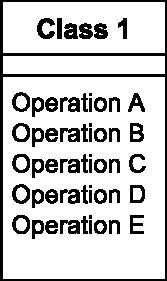
\includegraphics[width=\linewidth]{images/OriginalClassDiagram}
    \caption{origin}
    \label{fig:origin}
\end{subfigure}
\hfill
\begin{subfigure}[t]{0.2\linewidth}
    \centering
    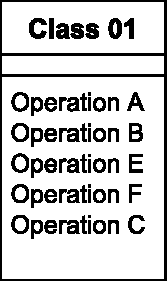
\includegraphics[width=\linewidth]{images/LeftClassDiagram}
    \caption{left}
    \label{fig:left}
\end{subfigure}
\hfill
\begin{subfigure}[t]{0.2\linewidth}
    \centering
    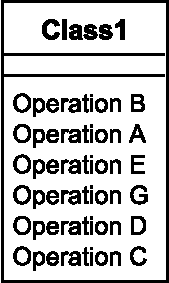
\includegraphics[width=\linewidth]{images/RightClassDiagram}
    \caption{right}
    \label{fig:right}
\end{subfigure}
\hfill
\label{fig:versions}
\caption{Different versions of a model.}
\end{figure}
\end{minipage}
\hfill
\begin{minipage}[t]{0.39\linewidth}
\begin{lstlisting}[style=eol,caption={The pseudo-formatted CBP of the model in Fig. \ref{fig:origin}.},label=lst:origincbp]
session "origin"
create c type Class
set c.name to "Class 1" 
create oa type Operation
set oa.name to "Operation A" 
create ob type Operation
set ob.name to "Operation B" 
create oc type Operation
set oc.name to "Operation C" 
create od type Operation
set od.name to "Operation D" 
create oe type Operation
set oe.name to "Operation E" 
add oa to c.operations at 0
add ob to c.operations at 1
add oc to c.operations at 2
add od to c.operations at 3
add oe to c.operations at 4
\end{lstlisting}
\end{minipage}

Change-based persistence is an alternative approach to the common state-based persistence (SBP) of models. Instead of persisting the last state of a model, CBP persists the overall history of changes of a model. For example, in SBP approach, when we save the UML class diagram in Fig. \ref{fig:origin} in standard XMI format, we only obtain the last state of the model the List. \ref{lst:originxmi} shows. In contrast, when we develop the model in CBP approach, a system captures all the changes made to the model and persists them into a CBP file as shown in List. \ref{lst:origincbp}\footnote{In implementation, the CBP is persisted in XML-like format, not in pseudo-format.}. The file consists of events generated by changes. Each event contains information about the type of the operation applied as well the as values, elements, or features involved. Replaying the events in List. \ref{lst:origincbp} produces the same model as in Fig. \ref{fig:origin}.

\section{Model Comparison}
\label{sec:model_comparison}
In a collaborative modelling setting, a model is commonly developed in parallel -- thus produces different versions. Let's say that the model in Fig. \ref{fig:origin} is modified by two different modellers in parallel. The first modeller produces the model in Fig. \ref{fig:left} (the left model), and the second one yields the model in Fig. \ref{fig:right} (the right model) producing XMI files as showed in List. \ref{lst:leftxmi} and List. \ref{lst:rightxmi} respectively.

\begin{minipage}[t]{0.49\linewidth} 
\begin{lstlisting}[style=eol,caption={The simplified XMI of the left model in Fig. \ref{fig:left}.},label=lst:leftxmi]
<uml:Class id="c" name="Class 01">
  <operation id="oa" 
    name="Operation A"/>
  <operation id="ob" 
    name="Operation B"/>
  <operation id="oe" 
    name="Operation E"/>
  <operation id="of" 
    name="Operation F"/>
  <operation id="oc" 
    name="Operation C"/>
</uml:Class>
\end{lstlisting}
\end{minipage}
\hfill
\begin{minipage}[t]{0.49\linewidth}
\begin{lstlisting}[style=eol,caption={The simplified XMI of the right model in Fig. \ref{fig:right}.},label=lst:rightxmi]
<uml:Class id="c" name="Class1">
  <operation id="ob" 
    name="Operation B"/>
  <operation id="oa" 
    name="Operation A"/>
  <operation id="oe" 
    name="Operation E"/>
  <operation id="og" 
    name="Operation G"/>
  <operation id="od" 
    name="Operation D"/>
  <operation id="oc" 
    name="Operation C"/>
</uml:Class>
\end{lstlisting}
\end{minipage}

At some point, these two models need to be compared (e.g. to identify their differences for analytics or conflicts when merging). The common approach to compare models is to create matches between the elements of both models and diff them. Generally, the matching process iterates through all the elements of the models being compared and matches them by their identifiers or through a similarity mechanism if they have none \cite{DBLP:conf/sfm/BroschKLSWW12,emfcompare2018developer}. After that, the diffing process then starts to find differences between the matched elements and their features\footnote{In default, the process iterates through all features, not only to the declared features in the XMI file, unless it has some mechanism to do so.}, commonly using the Longest Common Subsequence algorithms, e.g. \cite{DBLP:journals/algorithmica/Meyers86}. 

In our example, the matching iterates through all the elements of both model, 6 and 7 elements in the left and right models respectively, using their identifiers. The matching process yields 7 matches, $m_1$ = (\textsf{c}, \textsf{c}), $m_2$ = (\textsf{oa}, \textsf{oa}), $m_3$ = (\textsf{ob}, \textsf{ob}), $m_4$ = {\textsf{oe}, \textsf{oe}), (\textsf{of},), $m_5$ = (, \textsf{og}), $m_6$ = (, \textsf{od}), and $m_7$ = (\textsf{oc}, \textsf{oc}). The diffing process then iterates through all the matches and their features. In the first match, it identifies that both \textsf{c} elements are different in their \textsf{name} and \textsf{operations} features. The left \textsf{c}'s \textsf{name} is ``Class 01'' while the other \textsf{c}'s \textsf{name} is ``Class1'' (diff $d_1$).The \textsf{operations} features are different in their contents -- the positions of element \textsf{ob} are different in both features (diff $d_2$), the left \textsf{operations} feature contains element \textsf{of} that does not exist in the right \textsf{operations} (diff $d_3$}), and the left \textsf{operations} feature does not contain elements \textsf{og} and \textsf{od} (diffs $d_4$ and $d_5$) but exists in in the right \textsf{operations}. Other matches doe not have any differences.

Similar to EMF Compare \cite{emfcompare2018developer}, this paper presents differences as changes applied to a model so that it becomes equal to a reference model. These changes share a number of common elements: \textit{Match}, \textit{Feature}, \textit{Value}, \textit{Kind}, and \textit{Reference}. \textit{Match} is the match in which diffing is performed. Since elements' identifiers are used to match elements, the identifier is used to identify the match. \textit{Feature} and \textit{Value} are the feature and value involved in a change. \textit{Kind} is the type of the change. 
It can be one of these types: \textsf{CHANGE}, \textsf{ADD}, \textsf{DELETE}, and \textsf{MOVE}. \textsf{CHANGE} represents a change of value of a single attribute or non-containment reference. \textsf{ADD} represents an addition of a value to a multi-valued attribute, multi-valued non-containment reference, or single/multi-valued containment reference. \textsf{DELETE} is the counterpart of \textsf{ADD}. \textsf{MOVE} represents a change of position, containing feature, or container of a value. \textit{Reference} is the reference model. It can be the left or right model. For the rest of the paper, the left model is the reference model -- how to make the right model equals to the left model. 
    
Based on these definitions, we formalise the diffs identified previously as $d_n$ = [$Match_n$, $Feature_n$, $Value_n$, $Kind_n$]. Thus, $d_1$ =  [\textsf{c}, \textsf{name}, ``Change 01'', \textsf{CHANGE}], $d_2$ = [\textsf{c}, \textsf{operations}, \textsf{ob}, \textsf{MOVE}], $d_3$ = [\textsf{c}, \textsf{operations}, \textsf{of}, \textsf{ADD}],  $d_4$ = [\textsf{c}, \textsf{operations}, \textsf{og}, \textsf{DELETE}], and $d_5$ = [\textsf{c}, \textsf{operations}, \textsf{od}, \textsf{DELETE}]. Fig. \ref{fig:xmi_comparison} depicts the mapping of these diffs on the left and right models. Applying these diffs as changes to the right model will transform it into the left model.  
 \begin{figure}
     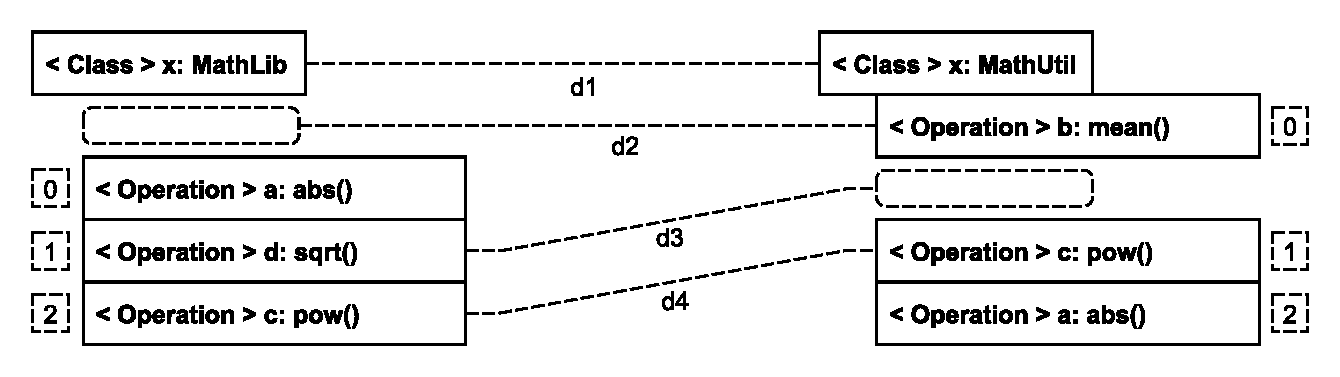
\includegraphics[width=\linewidth]{images/XmiComparison}
     \caption{A model comparison of the left and right models in Listings \ref{lst:leftxmi} and \ref{lst:rightxmi}.}
     \label{fig:xmi_comparison}
 \end{figure}
 

\section{Change-based Approach for Comparing Models}
\label{sec:change_based_approach_for_comparing_models}

 \begin{figure}
    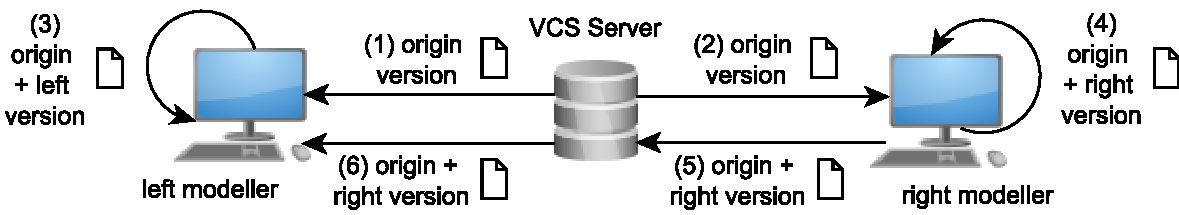
\includegraphics[width=\linewidth]{images/VCS}
    \caption{A case of the use of CBP in a collaborative modelling.}
    \label{fig:vcs}
\end{figure}

In the context of collaborative modelling using CBP, let's say that the file of the CBP in \ref{lst:origincbp} already exists in a text-based Version Control System (VCS) server (Fig. \ref{fig:vcs}). Both modellers checkout the original CBP (steps 1 and 2) and modify it (steps 3 and 4). Changes made by the left and right modellers will be appended to the original CBP producing two different CBP representation as displayed in Listings \ref{lst:leftcbp} and \ref{lst:rightcbp}\footnote{Both CBPs only present the changes after the last line of the original version (start from line 19). In implementation, the changes are appended to the original version.} -- capturing different courses of modification made by the modellers. The right developer then commits her work (original + right version) to the VCS. Since there is no new commit on the VCS, the commit process is straightforward (step 5). The left developer then decide to also commit his work (original + left version) to the VCS, thus his machine downloads the current version from the server (step 6). However, since the original version has been updated since his last checkout, he has to perform a model comparison to check the differences, and possibly conflicts, between his version (original + left version) and the updated original version (original + right version). 

\begin{minipage}[t]{0.49\linewidth}    
\begin{lstlisting}[firstnumber=19,style=eol,caption={The CBP of the model in Fig. \ref{fig:left} (left version).},label=lst:leftcbp]
session "LEFT"
set d.name from "Operation D" to "Op D"
set c.name from "Class 1" to "Class 01"
move oc in c.operations from 2 to 4
remove od from c.operations at 3
delete od
create of type Operation
set of.name to "Operation F"
add of to c.operations at 3
\end{lstlisting}
\end{minipage}
\hfill
\begin{minipage}[t]{0.49\linewidth}
\begin{lstlisting}[firstnumber=19,style=eol,caption={The CBP of the model in Fig. \ref{fig:right} (right version).},label=lst:rightcbp]
session "RIGHT"
set ob.name from "Operation B" to "Operation BB"
move oc in c.operations from 2 to 4
move oe in c.operations from 3 to 2
create og type Operation
set og.name to "Operation G" 
add og to c.operations at 3
move ob in c.operations from 1 to 0
set oa.name from "Operation BB" to "Operation B"
set c.name from "Class 1" to "Class1"
\end{lstlisting}
\end{minipage}

Since both modellers work using CBP, we can exploit the persistence to improve the previous model comparison. We do not need to visit and match element \textsf{ob} as it is affected by the recent changes in both CBPs, and also only the affected features by the recent changes that are compared -- not all features. 

In performing comparison, our approach has three phases: event loading, tree construction, and diff computation. These phases are represented as methods \textsf{loadEvents}, \textsf{contructObjectTree}, and \textsf{computeDifferences} methods in class \textsf{CBPComparison} in Fig. \ref{fig:approach_class_diagram}. 

\begin{figure}
    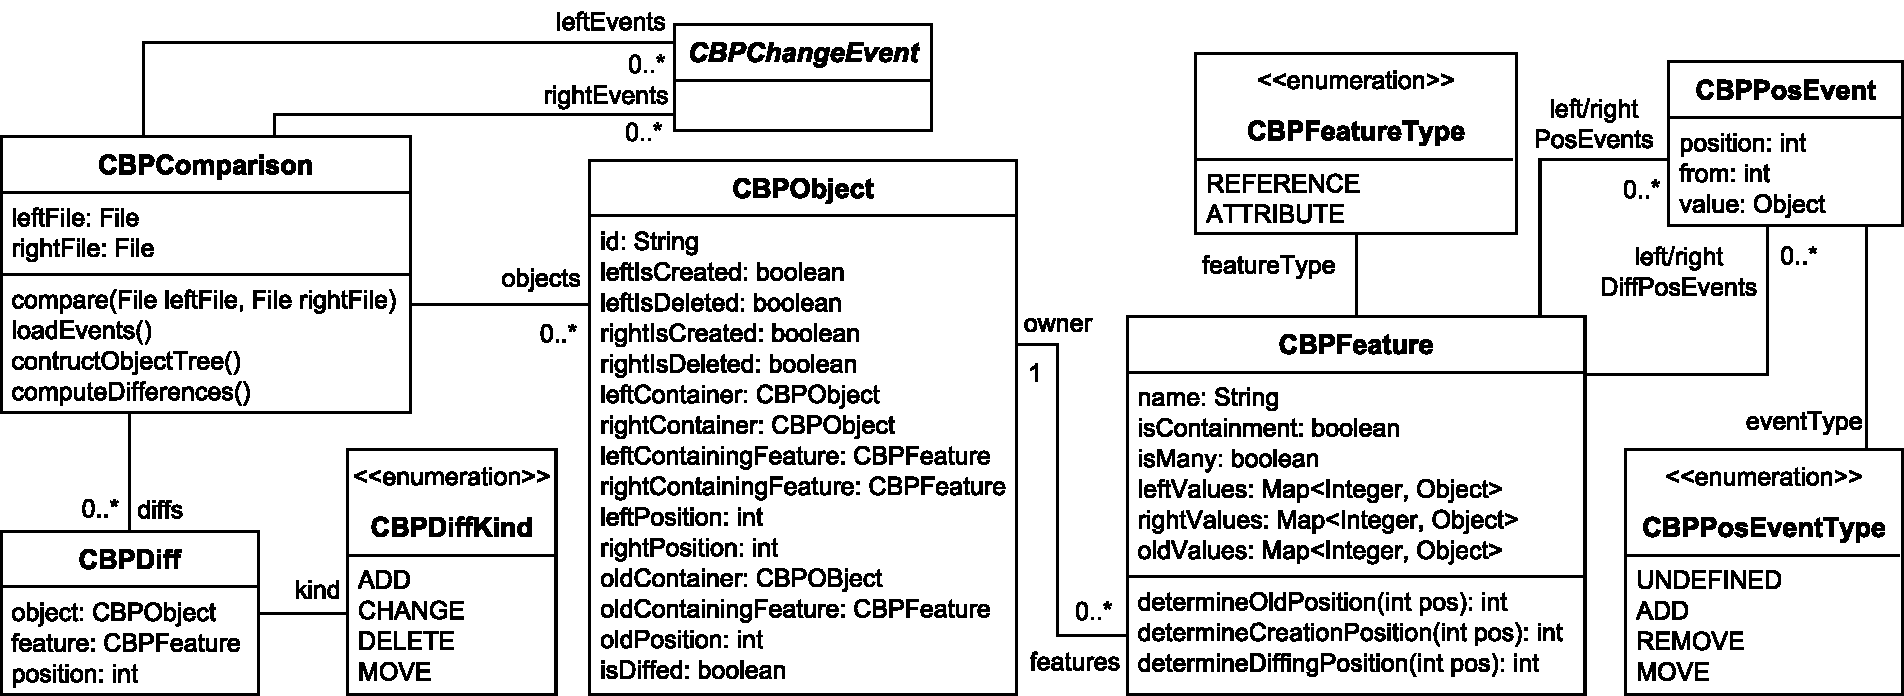
\includegraphics[width=\linewidth]{images/TreeClassDiagram}
    \caption{A class diagram showing the core components of the change-based approach to optimise model comparison.}
    \label{fig:approach_class_diagram}
\end{figure}

\subsection{Event Loading}
\label{sec:event_loading}
In the event loading, our implementation loads two supplied CBP files into memory as change-event instances of the class \textsf{CBPChangeEvent} in Fig. \ref{fig:approach_class_diagram}. Not all lines are converted into change events. Only lines starting from the position where the two files are different are loaded as change-events. In this case, lines 1-18 in List. \ref{lst:origincbp} are not loaded. Only lines starting from line 19 in Listings \ref{lst:leftcbp} and \ref{lst:rightcbp} are loaded, yielding two lists -- left and right -- of change-events. 

\subsection{Tree Construction}
\label{sec:tree_construction}
In the tree construction phase, our implementation iterates through both left and right change-event lists and construct an object tree based on the information available in each change-event. The object tree is similar to the list of matches in the previous model comparison except that, some of the differences, it has several flags (e.g.\textsf{*isCreated}, \textsf{*isDeleted} in class \textsf{CBPObject}, Fig. \ref{fig:approach_class_diagram}), it uses Map data structure instead of List (class \textsf{CBPFeature}, Fig. \ref{fig:approach_class_diagram}) to represent multi-valued features of the left and right models, and the presence of attribute \textsf{oldValues} to hold the original values of features. These specific traits are useful to determine differences in the diff computation phase.

\subsubsection{Left Side.}\label{sec:left_side} The iteration starts from the first line of the left CBP to the last line of the right CBP. The line 1 is a session event. Session event indicates that its following events -- until the next session event or end of file -- are one batch of changes when they were saved into a model persistence file. This event is not significant for model comparison, thus skipped.  



At line 2 of the left CBP (List. \ref{lst:leftcbp}), the \textsf{name} of element \textsf{od} is set from ``Operation D'' to ``Op D''. Using this information, we know that there is an element \textsf{od}, with its feature \textsf{name}, has been modified. Thus, a CBP object with id $od$ and a CBP feature $name$ is created. The value ``Op D'' is put to the $leftValues$ Map attribute of the CBP feature $name$ with $key$ = 0 indicating its position. Since \textsf{name} is a single-valued feature -- by looking at the model's metamodel, the $key$ is always 0. Also, the value ``Operation D'' is put to the $oldValues$ and $rightValues$ attributes of the CBP feature $name$ as its original value. 

Line 3 has the same change type of the first line. Thus, the same mechanism is also applied, producing a CBP object with id $c$ and a CBP feature $name$ with $leftValues$[0, ``Class 01''] (key = 0, value = ``Class 01''), $oldValues$[0, ``Class 1''], and $rightValues$[0, ``Class 1'']. At line 4, element \textsf{oc} in the \textsf{c}'s \textsf{operations} feature is moved from position 2 to 4. Thus, two CBP objects, $oc$ and $c$, are created, and a CBP feature $operations$ belongs to $c$ is also created. The $leftPosition$, $oldLeftPosition$, and $rightValues$ of $oc$ is set to 4, 2, and 2 respectively, which means $oc$ with  keys 4, 2, and 2 is also put to $leftValues$, $oldValues$, and $rightValues$ respectively. 

\begin{table}
    \centering
    \begin{footnotesize}
        \caption{The simplified state of the object tree after using the available information only from the left CBP to contruct it.}
        \label{table:left_object_tree}
        \begin{tabular}{  c  c  c  c  c  c  c  c  }
            \hline
            \multicolumn{3}{c}{Left} & \multirow{2}{*}{Objects} & \multicolumn{3}{c}{Right} & Origin\\
            \hhline{---~----}
            isCreated & isDeleted & leftValues & & rightValues & isCreated & isDeleted & oldValues\\
            \hline
            \rowcolor{gray1}
            false & false & & \textbf{\textsf{c}} & & false & false & \\
            \rowcolor{gray2}
            & & & \textbf{\textsf{name}} & & & & \\
            & & ``Class 01'' & \textbf{0} & ``Class 1'' & & & ``Class 1'' \\
            \rowcolor{gray2}
            & & & \textbf{\textsf{operation}} & & & & \\
            & & ?? & \textbf{\small{2}} & oc & & & oc \\
            & & of & \textbf{\small{3}} & od & & & od \\
            & & oc & \textbf{\small{4}} & ?? & & & ?? \\
            \hline
            \rowcolor{gray1}
            false & false & & \textbf{\textsf{oc}} & & false & false & \\
            \hline
            \rowcolor{gray1}
            false & \textbf{true} & & \textbf{\textsf{od}} & & false & false & \\
            \rowcolor{gray2}
            & & & \textbf{\textsf{name}} & & & & \\
            & & ``Op D'' & \textbf{0} & \makecell{``Opera\\tion D''} & & & \makecell{``Opera\\tion D''} \\
            \hline
            \rowcolor{gray1}
            \textbf{true} & false & & \textbf{\textsf{of}} & & false & false & \\
            \rowcolor{gray2}
            & & & \textbf{\textsf{name}} & & & & \\
            & & \makecell{``Opera\\tion F''} & \textbf{0} & & & &  \\
            \hline
        \end{tabular}
        \begin{flushright}
            \textit{grey}: object, \textit{light grey}: feature, \textit{white}: value, ??: the value is still unknown
        \end{flushright}
    \end{footnotesize}
\end{table}

At line 5, element \textsf{od} at index 2 is removed from \textsf{c}'s \textsf{operations} feature. Since the CBP objects of $od$ and $c$ already exists, there is no need to re-create them. Using the available information, CBP object $od$ is removed from $c$'s CBP Feature $operations$. As consequence, the position -- the key -- of CBP object $oc$ that already exists in the CBP feature is adjusted from 4 to 3. Line 6 deletes element \textsf{od} from the left model. To remember this deletion, the flag $leftIsDeleted$ in CBP object $od$ is set to $true$, indicating that $od$ has been existed since the original version but eventually deleted in the current version. 

Lines 7 to 9 create an \textsf{Operation} with id \textsf{of}, set its feature \textsf{name} to ``Operation F'', and add it to \textsf{c}'s feature \textsf{Operations} at position 3. As consequence, an CBP object $of$ is created. Its $leftIsCreated$ is set to $true$, indicating that the element is created in the current version. The CBP feature $name$ of $of$ is also created and its value is set to ``Operation F''. The CBP object $of$ then is added to $c$'s CBP feature $operations$ at position 3, moving the CBP object $oc$ from position 3 back to 4. 

The state of the object tree after using the available information in the left CBP to construct it is summarised in Table \ref{table:left_object_tree}. The grey, light grey, and white lines represent CBP object, CBP feature, and value respectively. The values of CBP feature $operations$ refer/point to the respective CBP objects. The `??' symbol indicates that the value at its position is still unknown.

\subsubsection{Right Side.} \label{sec:right_side} The iteration continues to the right CBP. The line 1 is skipped since it is a session event.  At line 2, a CBP object with id $ob$ and CBP feature $name$ is created. The values of CBP feature $name$ are also set so that it has $rightValues$[0, ``Operation BB''], $oldValues$[0, ``Operation B''], and $leftValues$[0, ``Operation B'']. 

\begin{table}
    \centering
    \begin{footnotesize}
        \caption{The simplified state of the object tree after using the available information from both \textbf{left and right} CBPs to contruct it.}
        \label{table:right_object_tree}
        \begin{tabular}{  c  c  c  c  c  c  c  c  }
            \hline
            \multicolumn{3}{c}{Left} & \multirow{2}{*}{Objects} & \multicolumn{3}{c}{Right} & Origin\\
            \hhline{---~----}
            isCreated & isDeleted & leftValues & & rightValues & isCreated & isDeleted & oldValues\\
            \hline
            \rowcolor{gray1}
            false & false & & \textbf{\textsf{c}} & & false & false & \\
            \rowcolor{gray2}
            & & & \textbf{\textsf{name}} & & & & \\
            & & ``Class 01'' & \textbf{0} & ``Class 1'' & & & ``Class 1'' \\
            \rowcolor{gray2}
            & & & \textbf{\textsf{operation}} & & & & \\
            & & ?? & \textbf{\small{0}} & oc & & & ?? \\
            & & ob & \textbf{\small{1}} & ?? & & & ob \\
            & & oe & \textbf{\small{2}} & oe & & & oc \\
            & & of & \textbf{\small{3}} & og & & & od \\
            & & oc & \textbf{\small{4}} & od & & & oe \\
            & & ?? & \textbf{\small{5}} & oc & & & ?? \\
            \hline
            \rowcolor{gray1}
            false & false & & \textbf{\textsf{oc}} & & false & false & \\
            \hline
            \rowcolor{gray1}
            false & \textbf{true} & & \textbf{\textsf{od}} & & false & false & \\
            \rowcolor{gray2}
            & & & \textbf{\textsf{name}} & & & & \\
            & & ``Op D'' & \textbf{0} & \makecell{``Opera\\tion D''} & & & \makecell{``Opera\\tion D''} \\
            \hline
            \rowcolor{gray1}
            \textbf{true} & false & & \textbf{\textsf{of}} & & false & false & \\
            \rowcolor{gray2}
            & & & \textbf{\textsf{name}} & & & & \\
            & & \makecell{``Opera\\tion F''} & \textbf{0} & & & &  \\
            \hline
            \rowcolor{gray1}
            false & false & & \textbf{\textsf{oe}} & & false & false & \\
            \hline
            \rowcolor{gray1}
            false & false & & \textbf{\textsf{ob}} & & false & false & \\
            \rowcolor{gray2}
            & & & \textbf{\textsf{name}} & & & & \\
            & & \makecell{``Opera\\tion B''} & \textbf{0} & \makecell{``Opera\\tion B''} & & & \makecell{``Opera\\tion B''}\\
            \hline
            \rowcolor{gray1}
            false & false & & \textbf{\textsf{og}} & & \textbf{true} & false & \\
            \rowcolor{gray2}
            & & & \textbf{\textsf{name}} & & & & \\
            & &  & \textbf{0} & \makecell{``Opera\\tion G''} & & & \\
            \hline
        \end{tabular}
        \begin{flushright}
            \textit{grey}: object, \textit{light grey}: feature, \textit{white}: value, ??: the value is still unknown
        \end{flushright}
    \end{footnotesize}
\end{table}

\subsection{Diff Computation}
\label{sec:diff_computation}

\section{Evaluation}
\label{sec:evaluation}

Explain the procedure.

Comparison using CBP is much faster than traditional state-based comparison.

Relationship between number of diffs, number of elements, number of events, and comparison time of CBP and SBP. See the $R^2$.

Too much events slowdowns CBP.
 
\begin{figure}
\hfill
\centering    
\begin{subfigure}{\linewidth}
    \centering
    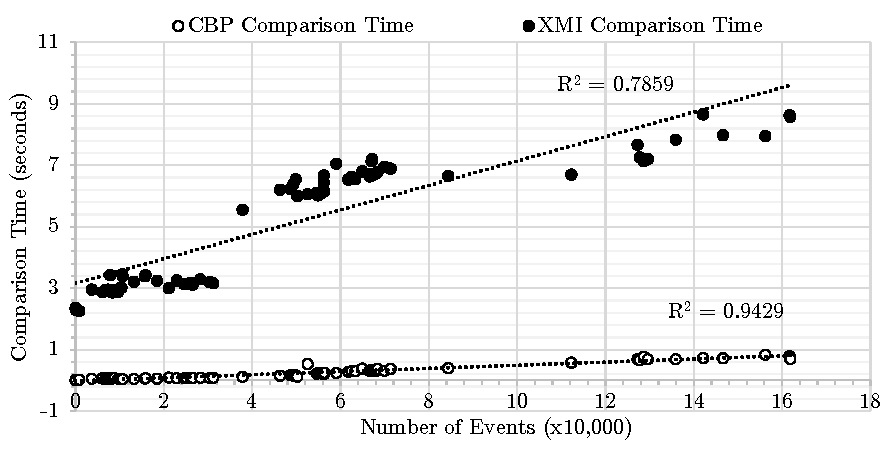
\includegraphics[width=\linewidth]{images/Time-Events}
    \caption{comparison time vs. number of events}
    \label{fig:time_events}
\end{subfigure}
\hfill
\centering    
\begin{subfigure}{\linewidth}
    \centering
    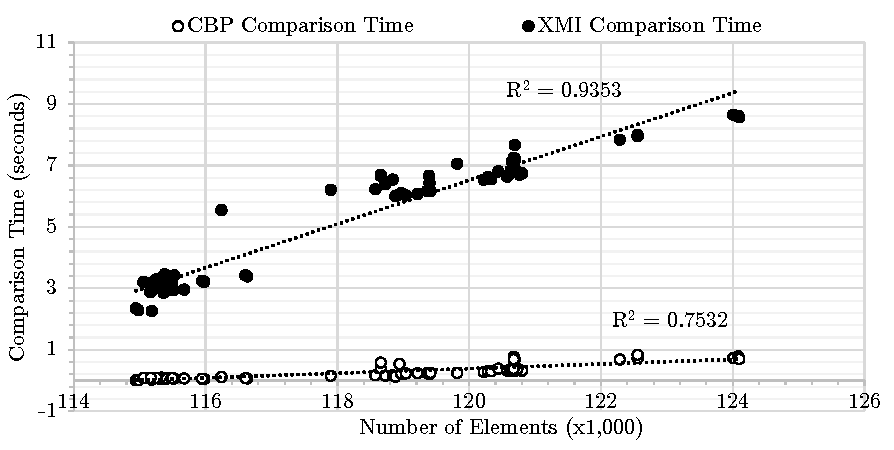
\includegraphics[width=\linewidth]{images/Time-Elements}
    \caption{comparison time vs. number of elements}
    \label{fig:time_elements}
\end{subfigure}
\\
\hfill
\centering    
\begin{subfigure}{\linewidth}
    \centering
    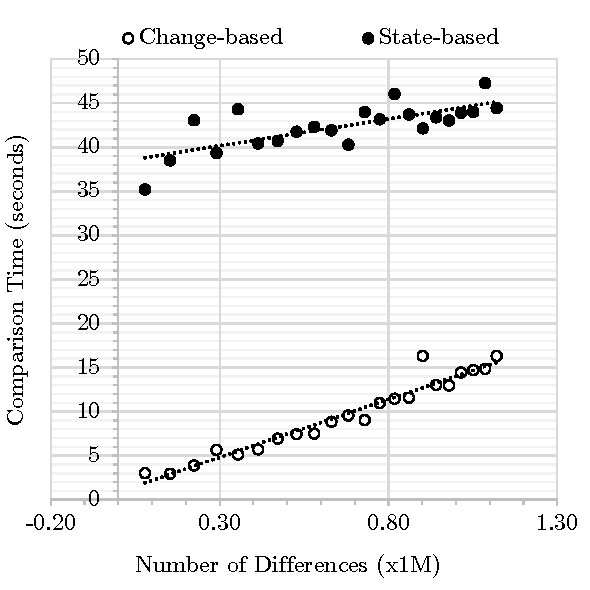
\includegraphics[width=\linewidth]{images/Time-Diffs}
    \caption{comparison time vs. number of diffs}
    \label{fig:time_diffs}
\end{subfigure}
\hfill
\label{fig:perfomance_evaluation}
\caption{Comparison between CBP and XMI on model comparison time.}
\end{figure}

\subsection{Limitation and Threat to Validity}
\label{sec:limitation_and_Threat_to_validity}

Heavily relies on identifiers.

model size.

changes may not reflect real-word changes.



\section{Related Work}
\label{sec:related_work}

EMF Compare, SiDiff, ECL. Comparison at the structural level. 

EMFStore. Comparison at the change/operational level. 

Our approach use the information at the change level to identify differences at the structural level.


\section{Conclusions and Future Work}
\label{sec:conclusion_and_future_work}

Future work: Use the CBP for model merging.

\vspace{-10pt}
\subsubsection*{Acknowledgements.} This work was partly supported by through a scholarship managed by \emph{Lembaga Pengelola Dana Pendidikan Indonesia} (Indonesia Endowment Fund for Education).
%\clearpage

\bibliography{references} 
\bibliographystyle{splncs}

\end{document} 
